\documentclass[oneside, 11pt]{article}

\usepackage[T1]{fontenc}
\usepackage[utf8]{inputenc}
\usepackage[english]{babel}

\usepackage{fouriernc}
\usepackage[detect-all, binary-units, separate-uncertainty=true,
            per-mode=symbol, retain-explicit-plus, retain-unity-mantissa=false]{siunitx}

\usepackage{setspace}
\setstretch{1.2}

\setlength{\parskip}{\smallskipamount}
\setlength{\parindent}{0pt}

\usepackage[headheight=14pt]{geometry}
\geometry{marginparwidth=0.5cm, verbose, a4paper, tmargin=3cm, bmargin=3cm,
          lmargin=2cm, rmargin=2cm}

\usepackage{float}

\usepackage[fleqn]{amsmath}
\numberwithin{equation}{section}
\numberwithin{figure}{section}

\usepackage{graphicx}
\graphicspath{{images/}{../../../images/}}

\usepackage{tikz}
\usetikzlibrary{shapes}
\usetikzlibrary{plotmarks}

\newcounter{Exercise}
\setcounter{Exercise}{1}
\usepackage{xcolor}
\definecolor{shadecolor}{gray}{0.9}
\usepackage{framed}
\usepackage{caption}

\usepackage{url}


\usepackage{fancyhdr}
\pagestyle{fancy}
\fancyhf{}
\rhead{\thepage}
\renewcommand{\footrulewidth}{0pt}
\renewcommand{\headrulewidth}{0pt}

\fancypagestyle{firststyle}
{
    \fancyhf{}
    \rhead{\thepage}
    \cfoot{
\includegraphics[height=30pt]{HiSPARClogo}}
    \rfoot{
\includegraphics[height=25pt]{CCbysa}}
    \lfoot{
\includegraphics[height=30pt]{NIKHEFlogo}}
    \renewcommand{\footskip}{50pt}
    \renewcommand{\footrulewidth}{0.1pt}
    \renewcommand{\headrulewidth}{0pt}
}

\newcommand{\figref}[1]{Figuur~\ref{#1}}

\newcommand{\hisparc}{\textsmaller{HiSPARC}\xspace}
\newcommand{\kascade}{\textsmaller{KASCADE}\xspace}
\newcommand{\sapphire}{\textsmaller{SAPPHiRE}\xspace}
\newcommand{\jsparc}{\textsmaller{jSparc}\xspace}
\newcommand{\hdf}{\textsmaller{HDF5}\xspace}
\newcommand{\aires}{\textsmaller{AIRES}\xspace}
\newcommand{\csv}{\textsmaller{CSV}\xspace}
\newcommand{\python}{\textsmaller{PYTHON}\xspace}
\newcommand{\corsika}{\textsmaller{CORSIKA}\xspace}
\newcommand{\labview}{\textsmaller{LabVIEW}\xspace}
\newcommand{\daq}{\textsmaller{DAQ}\xspace}
\newcommand{\adc}{\textsmaller{ADC}\xspace}
\newcommand{\hi}{\textsc{h i}\xspace}
\newcommand{\hii}{\textsc{h ii}\xspace}
\newcommand{\mip}{\textsmaller{MIP}\xspace}
\newcommand{\hisparcii}{\textsmaller{HiSPARC II}\xspace}
\newcommand{\hisparciii}{\textsmaller{HiSPARC III}\xspace}

\DeclareSIUnit{\electronvolt}{\ensuremath{\mathrm{e\!\!\:V}}}

\DeclareSIUnit{\unitsigma}{\ensuremath{\sigma}}
\DeclareSIUnit{\mip}{\textsmaller{MIP}}
\DeclareSIUnit{\adc}{\textsmaller{ADC}}

\DeclareSIUnit{\gauss}{G}
\DeclareSIUnit{\parsec}{pc}
\DeclareSIUnit{\year}{yr}



\begin{document}

\title{Data verwerking zonder periodieke afhankelijkheid}
\author{N.G. Schultheiss}
\date{}

\maketitle
\thispagestyle{firststyle}

\section{Inleiding}

Deze module volgt op de module ``Data verwerking met periodieke
afhankelijkheid'', waarin werd uitgelegd hoe je een spreadsheet met
gegevens van de detectoren kunt maken. Hier werd uitgelegd hoe
conclusies te trekken zijn, als er sprake is van een periodieke
afhankelijkheid. In het geval van de afhankelijkheid van
weersverschijnselen zoals bliksem, zal dit niet periodiek zijn. Het is
namelijk niet zo dat er om een bepaalde tijd een bliksemflits wordt
gegenereerd. 


\section{De opstelling}

Een opstelling die bijvoorbeeld op school gebruikt wordt, bestaat uit
(groepen van) twee detectoren. Om een shower van de achtergrondstraling
te isoleren, zoeken we coincidenties. Dit wil zeggen dat er (praktisch)
tegelijk deeltjes in de twee verschillende detectoren worden
gedetecteerd. De shower wordt boven in de atmosfeer gestart door de
botsing van kosmische straling met kerndeeltjes \footnote{Verwijzing
naar {}``Interactie van kosmische straling en aardatmosfeer''.}. Deze
botsing veroorzaakt een kettingreactie, waardoor een shower van deeltjes
door de atmosfeer gaat. Een deel van deze shower wordt in de atmosfeer
geabsorbeerd, een deel komt op Aarde bij de detector. In de praktijk
kunnen we zeggen dat de deeltjes bijna loodrecht op de Aarde vallen, de
hoek van inval is meestal kleiner dan $20^{o}$ met het zenith
\footnote{Het zenith is het punt recht boven je hoofd. Ieder mens (en
iedere plaats) heeft een eigen zenith.}.

\begin{figure}[h]
\centering

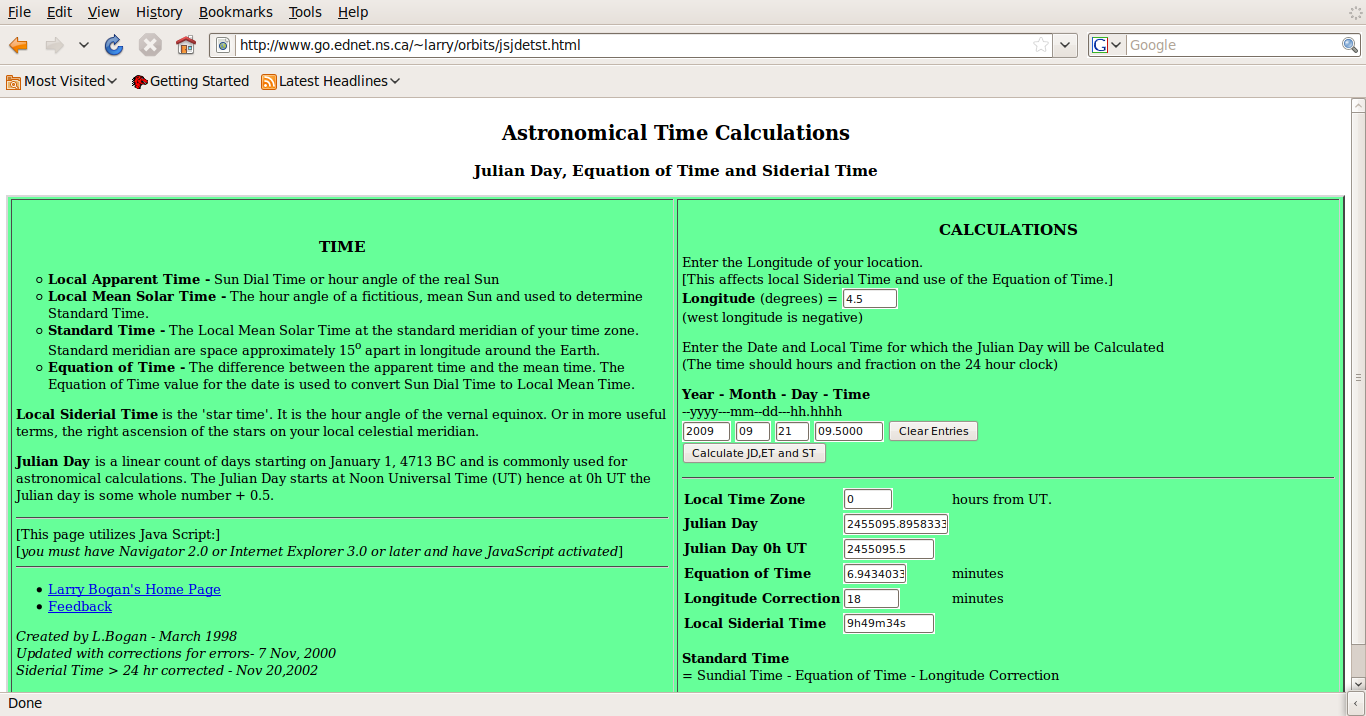
\includegraphics[width=16cm]{Astronomical_Time_Calculations}

\caption{Een conversie pagina}
\end{figure}


Omdat de Aarde ronddraait, draaien de detectoren ook rond. Zoals we
in de module {}``De Hemel'' kunnen zien, is dit draaien van de Aarde
ten opzichte van de Zon of ten opzichte van de sterren te beschouwen.
De gegevens worden aangeleverd met de Aardse tijd. De draaiing van
de Aarde wordt hier dus gegeven ten opzichte van de Zon. Soms willen
we de metingen echter hebben in siderische tijd of ten opzichte van
de sterren. Een conversiepagina is met google te vinden, zoals:

http://www.go.ednet.ns.ca/\textasciitilde{}larry/orbits/jsjdetst.html


\section{Gegevens ophalen}

Gegevens kunnen opgehaald worden op: http://data.hisparc.nl/. Er
verschijnt een lijst met station locaties. Klik je op een station, dan
krijg je een pagina met de gegevens van die detectoren. Van boven naar
beneden zie je een histogram met het aantal coïncidenties per uur, een
grafiek met het aantal pulsen tegen de pulshoogte in mV (millivolt) en
een grafiek met het aantal pulsen tegen het oppervlak van de puls in
mVns (millivolt nanoseconde).

Rechts naast de grafieken is een kolom met daarin de datum van de
metingen en verschillende eigenschappen van het meetstation zoals
breedte- (latitude) en lengtegraad (longitude).

Rechts boven de grafieken is {}``Source'' te zien, klik je hierop
dan krijg je een {*}.csv (comma separated values) bestand. Dit is
in een spreadsheet programma te laden. Soms moet je aangeven dat de
informatie door komma's gescheiden is.

\begin{figure}[h]
\centering

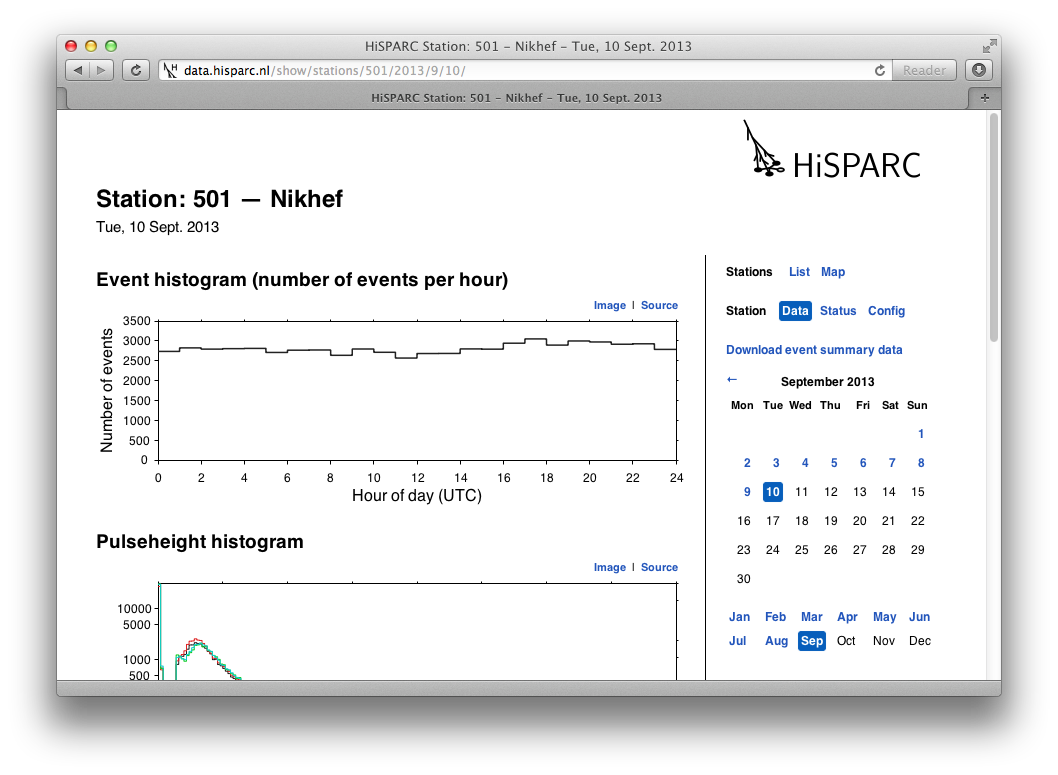
\includegraphics[width=14cm]{HiSPARC_Public_Database}

\caption{Het data venster}
\end{figure}


Nu deze gegevens bekend zijn, kunnen we onderzoeken of deze gegevens
afhangen van andere grootheden. 

\end{document}
